\begin{figure*}[ht]
\centering
    \centering
    \begin{subfigure}[b]{0.39\textwidth}
            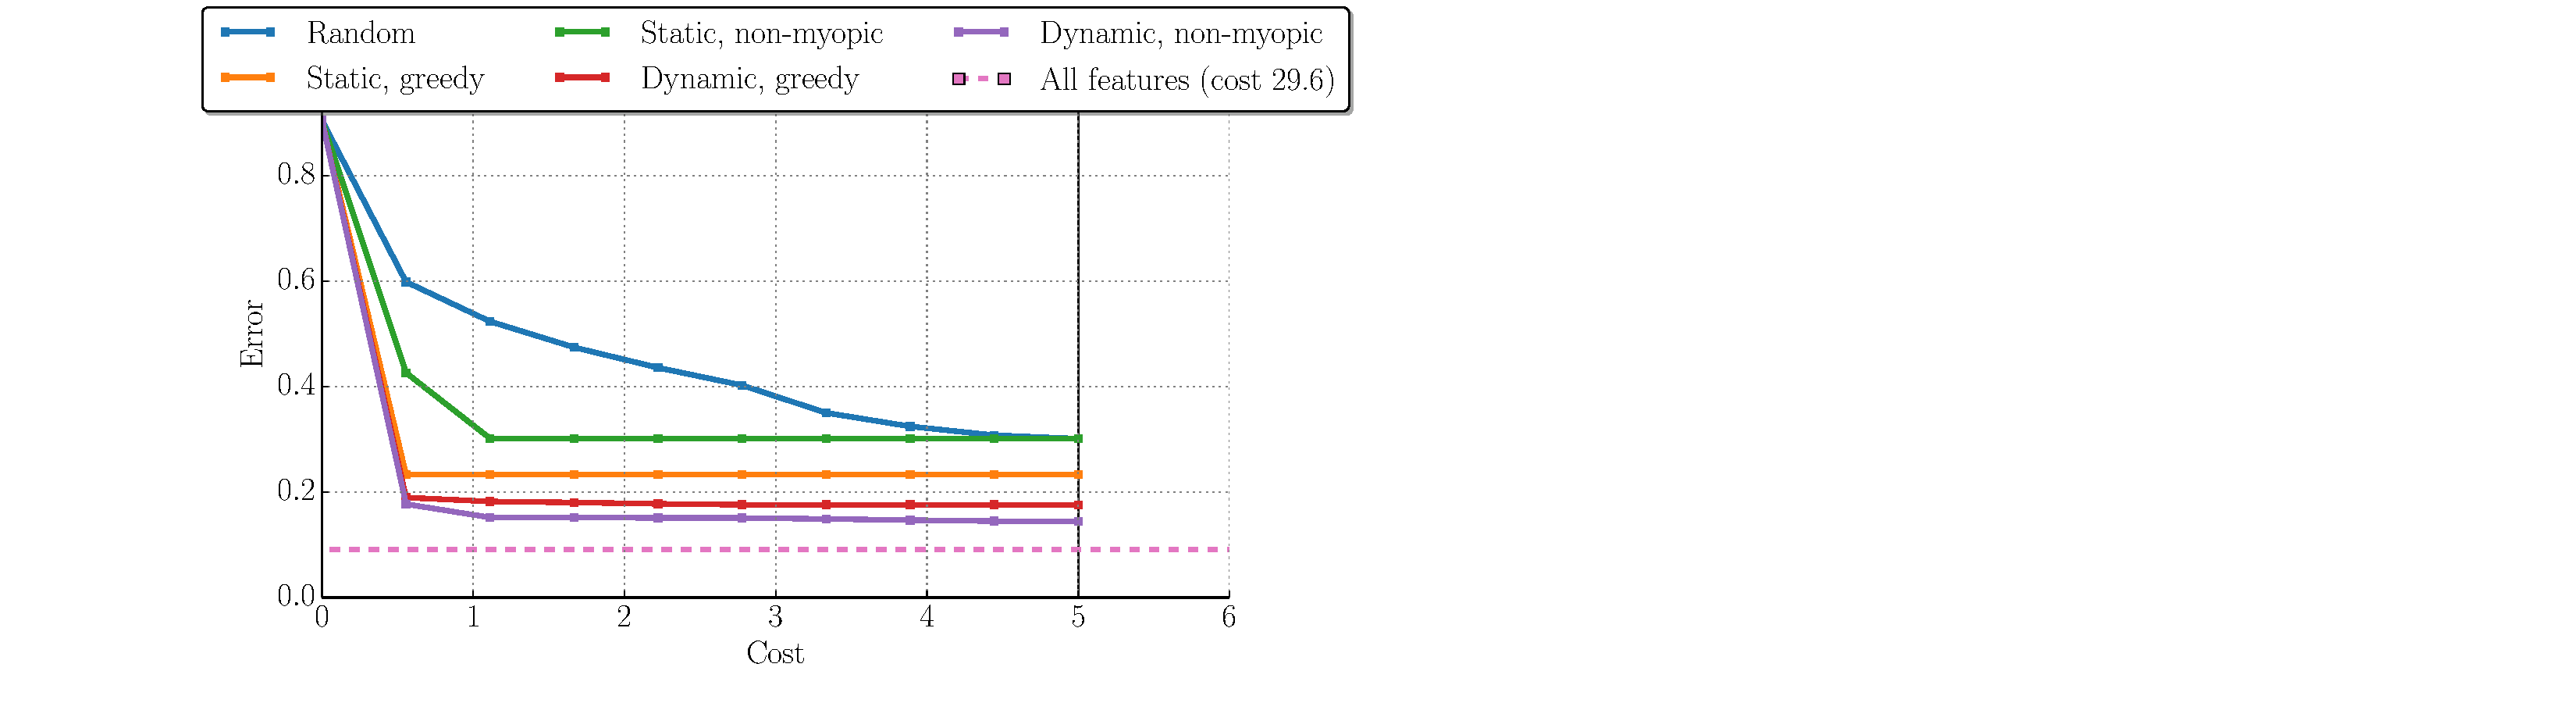
\includegraphics[width=\textwidth]{../../figures/apr11_assembly/scene_15_5_crop.pdf}
            \caption{Error given by policies learned for a budget = 5.}
    \end{subfigure}%
    \begin{subfigure}[b]{0.36\textwidth}
            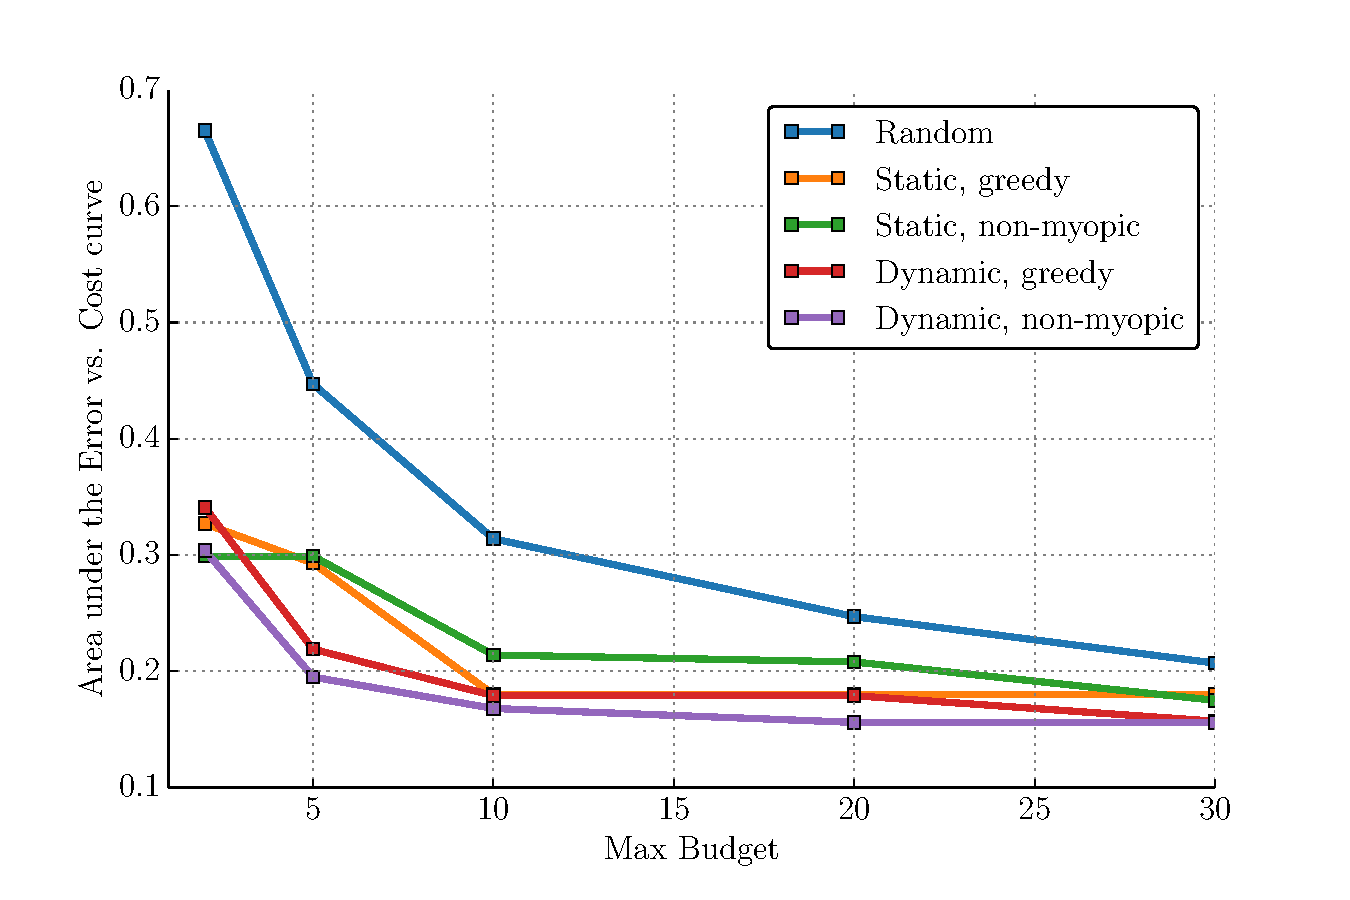
\includegraphics[width=\textwidth]{../../figures/apr11_assembly/_scenes15_auc.pdf}
            \caption{Areas under error vs. cost curves of policies learned at different budgets.}
    \end{subfigure}%
    \begin{subfigure}[b]{0.25\textwidth}
            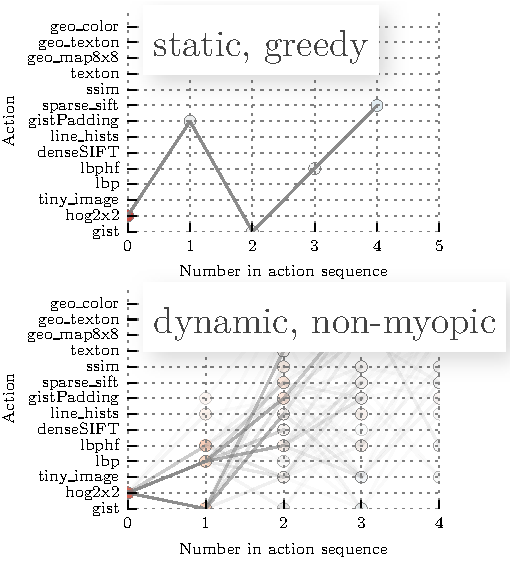
\includegraphics[width=\textwidth]{../../figures/apr11_assembly/scenes_result.pdf}
            \caption{Policy trajectories.}
    \end{subfigure}

    \caption{
Results on Scenes-15 dataset (best viewed in color).
Figure (a) shows the error vs. cost plot for policies learned given a budget of 5 seconds.
Figure (b) aggregates the area under the error vs. cost plot metrics for different policies and budgets, showeing that our approach outperforms baselines no matter what budget it's trained for.
Figure (c) shows the branching behavior of our dynamic policy.
}\label{fig:scenes}
\end{figure*}
